%%%%%%%%%%%%%%%%%%%%%%%%%%%%%%%%%%%%%%%%%%%%%%%%%%%%%%%%%%%%%%%%%%%%%%%
%%%%%%%%%%%%%%%%%%%%%%%%%%%%%%%%%%%%%%%%%%%%%%%%%%%%%%%%%%%%%%%%%%%%%%%
%%%%%%%%%%%%%%%%%%%%%%%%%%%%%%%%%%%%%%%%%%%%%%%%%%%%%%%%%%%%%%%%%%%%%%%


% \subsection{Existing works on temporal graph learning}

\noindent\textbf{Preliminary.}
Figure~\ref{fig:temporal_graph_with_feats} is an illustration on the temporal graph.
Our goal is to predict whether two nodes are connected at a specific timestamp $t_0$ based on all the available temporal graph information happened before that timestamp.
For example, to predict whether $v_1, v_2$ are connected at $t_0$, we only have access to the graph structure, node features, and link features with timestamps from $t_1$ to $t_6$.

\begin{figure}[t]
    \centering
    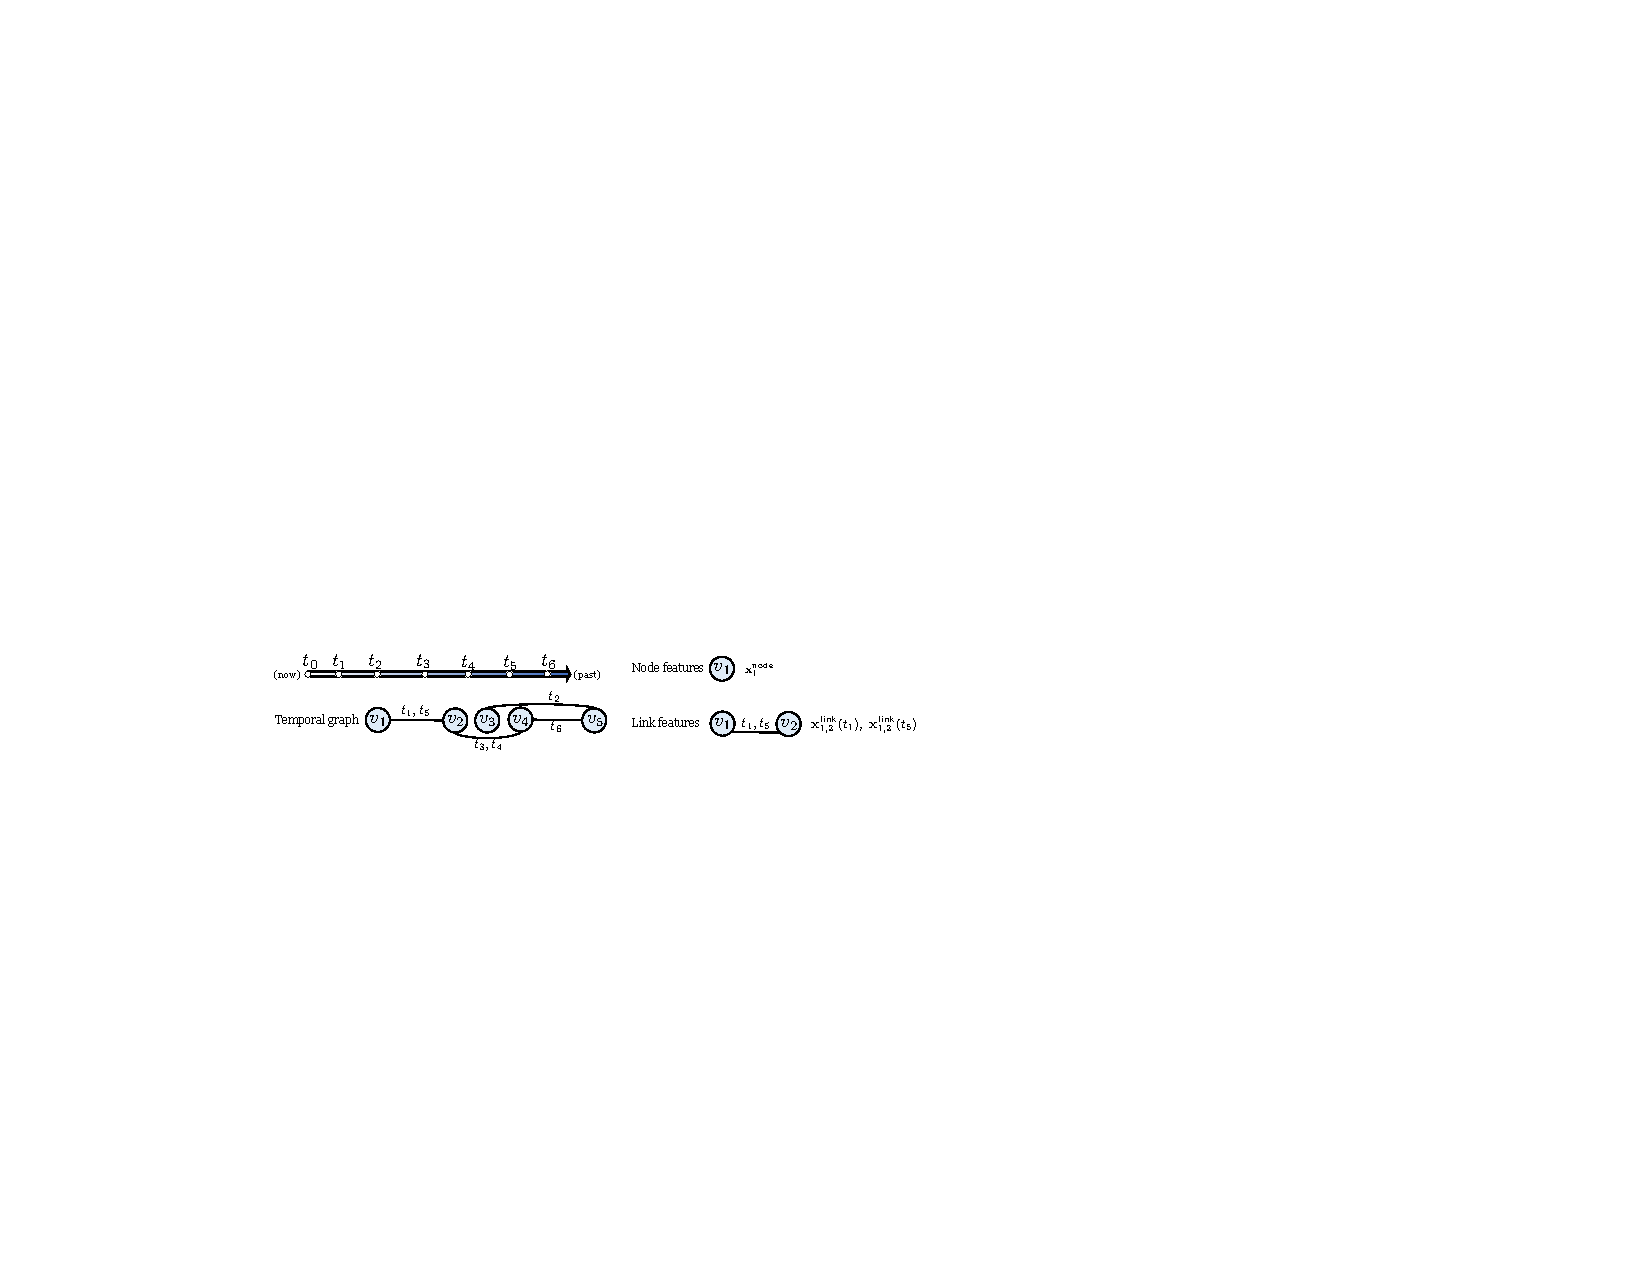
\includegraphics[width=0.99\textwidth]{figures/temporal_graph_with_feats.pdf}
    \vspace{-3mm}
    \caption{(Left) Temporal graph with nodes $v_1,\ldots, v_5$, per-link timestamps $t_1,\ldots,t_6$ indicate when two nodes interact. For example, $v_1, v_2$ interact at $t_1, t_5$.  (Right) Each node has its node features (e.g., $\mathbf{x}_1^\text{node}$ for $v_1$) and each temporal link has its link features (e.g., $\mathbf{x}_{1,2}^\text{link}(t_1), \mathbf{x}_{1,2}^\text{link}(t_5)$ are link features between $v_1, v_2$ at $t_1,t_5$). For scenarios without node or link features, we use all-zero vectors instead.
    % (Application) In link prediction, we want to predict whether link exists at $t_0$ based on the historical node interactions.
    }
    \label{fig:temporal_graph_with_feats}
    \vspace{-3mm}
\end{figure}

\noindent\textbf{Related works.} 
Most of the temporal graph learning methods are conceptually and technically complicated with advanced neural architectures.
It is non-trivial to fully understand the algorithm details without looking into their implementations.
Therefore, we select the four most representative and most closely-related methods to introduce and compare them in more details.
\begin{itemize} [noitemsep,topsep=0pt,leftmargin=5mm ]
\item \noindent\textit{\textbf{JODIE}}~\cite{kumar2019predicting} is a \emph{RNN-based method}.
% , where the temporal neighbors are defined as \emph{the most recent interacted node}.
Let us denote $\mathbf{x}_i(t)$ as the embedding of node $v_i$ at time $t$, $\mathbf{x}_{ij}^\text{link}(t)$ as the link feature between $v_i,v_j$ at time $t$, and $m_i$ as the timestamp that $v_i$ latest interact with other node.
JODIE pre-processes and updates the representation of each node via RNNs (is it just one RNN or multiple RNNs).
More specifically, when an interaction between $v_i, v_j$ happens at time $t$, JODIE updates the temporal embedding using RNN by
\smash{$\mathbf{x}_i(t) = \texttt{RNN}\left(\mathbf{x}_i(m_i), \mathbf{x}_j(m_j), \mathbf{x}_{ij}^\text{link}(t), t-m_i \right)$.}
Then, the dynamic embedding of node $v_i$ at time $t_0$ is computed by $\mathbf{h}_i(t_0) = \left(1 + (t_0-m_i) \mathbf{w} \right) \cdot \mathbf{x}_i(m_i)$.
Finally, the prediction on any node pair at time $t_0$ is computed by $\texttt{MLP}([\mathbf{h}_i(t_0)~||~ \mathbf{h}_j(t_0)]) $, where $[\cdot||\cdot]$ is the concatenate operation and $\texttt{MLP}(\mathbf{x})$ is applying 2-layer MLP on $\mathbf{x}$.

\item \noindent\textit{\textbf{DySAT}}~\cite{sankar2020dysat} is a \emph{SAM-based method}. DySAT requires pre-processing the temporal graph into multiple snapshot graphs by first splitting all timestamps into multiple time-slots, then merging all edges in each time-slot.
% and the temporal neighbors are defined as \emph{$2$-hop uniform sampled neighbors}. 
Let $\mathcal{G}_t(\mathcal{V}, \mathcal{E}_t)$ denote the $t$-th snapshot graph. 
To capture spatial information, DySAT first applies Graph Attention Network (GAT)~\cite{velivckovic2018graph} on each snapshot graph $\mathcal{G}_t$ independently by $\mathbf{X}(t) = \texttt{GAT}(\mathcal{G}_t)$.
Then, to capture of temporal information for each node, Transformer is applied to $\mathbf{x}_i(t) = [\mathbf{X}(t)]_i$ at different timestamps to capture the temporal information by
\smash{$\mathbf{h}_i(t_k),\ldots \mathbf{h}_i(t_0)  = \texttt{Transformer}\big(\mathbf{x}_i(t_k), \ldots, \mathbf{x}_i(t_0) \big).$}
Finally, the prediction on any node pair at time $t_0$ is computed by $\texttt{MLP}([\mathbf{h}_i(t_0)~||~ \mathbf{h}_j(t_0)]) $. 

\item \noindent\textit{\textbf{TGAT}}~\cite{xu2020inductive} is a \emph{SAM-based method} that could capture the spatial and temporal information simultaneously.
% , where the temporal neighbors are defined as \emph{$2$-hop uniform sampled neighbors}..
TGAT first generates the time augmented feature of node $i$ at time $t$ by concatenating the raw feature $\mathbf{x}_i$ with a trainable time encoding $\mathbf{z}(t)$ of time $t$, i.e.,
$ \mathbf{x}_i(t) = [\mathbf{x}_i~||~ \mathbf{z}(t)]$ and $\mathbf{z}(t) = \cos( t \mathbf{w} + \mathbf{b})$.
Then, SAM is applied to the time augmented features and produces node representation 
$\mathbf{h}_i(t_0)= \texttt{SAM}\left(\mathbf{x}_i(t_0), \left\{\mathbf{x}_u(h_u)~|~u\in\mathcal{N}_{t_0}(i) \right\}\right)$, where $\mathcal{N}_{t_0}(i)$ denotes the neighbors of node $i$ at time $t_0$ and $h_u$ denotes the timestamp of the latest interaction of node $u$.
Finally, the prediction on any node pair at time $t_0$ is computed by $\texttt{MLP}([\mathbf{h}_i(t_0)~||~ \mathbf{h}_j(t_0)]) $.

\item \noindent\textit{\textbf{TGN}}~\cite{tgn_icml_grl2020} is a mixture of \emph{RNN- and SAM-based method}. 
% , where the temporal neighbors ar e defined as \emph{$1$-hop most recent neighbors}.
In practice, TGN first captures the temporal information using RNN (similarly to JODIE), and then applies graph attention convolution to capture the spatial and temporal information jointly (similarly to TGAT).
\end{itemize}

Besides, we also consider the following temporal graph learning methods as baselines. These methods could be thought of as an extension on top of the above four most representative methods, but with the underlying idea behind the model design much more conceptually complicated.
\textit{\textbf{CAWs}}~\cite{wang2020inductive} is a mixer of \emph{RNN- and SAM- based method} that proposes to represent network dynamics by extracting temporal network motifs using temporal random walks.
CAWs  replaces node identities with the hitting counts of the nodes based on a set of sampled walks to establish the correlation between motifs. Then, the extracted motifs are fed into RNNs to encode each walk as a representation, and use SAM to aggregate the representations of multi-walks into a single vector for downstream tasks.
\textit{\textbf{TGSRec}}~\cite{fan2021continuous} is a \emph{SAM-based method} that proposes to unify sequential patterns and temporal collaborative signals to improve the quality of recommendation. To achieve this goal, they propose to advance the SAM by adopting novel collaborative attention, such that SAM can simultaneously capture collaborative signals from both users and items, as well as consider temporal dynamics inside sequential patterns.
\textit{\textbf{APAN}}~\cite{wang2021apan} is a \emph{RNN-based method} that proposes to decouple model inference and graph computation to alleviate the damage of the heavy graph query operation to the speed of model inference.
More related works are deferred to Appendix~\ref{section:other_related_work}.


% Specif- ically, we explicitly encode short-term preference and opti-
% mize it via memory mechanism, which has three key opera- tions: Message, Aggregate and Update. Our memory mech- anism can not only store one-hop information, but also trig- ger with new interactions online.,
% \begin{table}[t]
% \centering
% \begin{tabular}{ l l l l l l }
% \hline
%                   & JODIE & DySAT & TGAT & TGN & Ours \\ \hline \hline
% Key mechanism     & RNN  & SAM   & SAM  & RNN + SAM & MLP \\ 
% Sampling methods  &       &       &      &     &      \\  
% Use time-encoding &       &       &      &     &      \\ \hline\hline
% \end{tabular}
% \end{table}



